\documentclass[12pt]{article}
\usepackage{graphicx}
\usepackage{dblfloatfix}

\begin{document}
	
\section{PROGRAMMING LANGUAGES}
 
\subsection{TYPES OF PROGRAMMING LANGUAGES}

\begin{itemize}                                         
	\item Python                         
	\item C++                            
	\item Java
	\item JavaScript
	\item HTML
\end{itemize}

\begin{figure}[h]
		\
		
\includegraphics[width=0.7\linewidth]{bababooey}
		\caption{image via:dummies.com}
		\label{fig:bababooey}
\end{figure}

\newpage

\section{History of python programming language}

\begin{itemize}
           \item In the late 1980s Guido van Rossum designed python.
           \item It was released firstly on the 20th of february.
           \item Python Software Foundation helped in the development of the language.

\end{itemize}

\begin{figure}[h]
	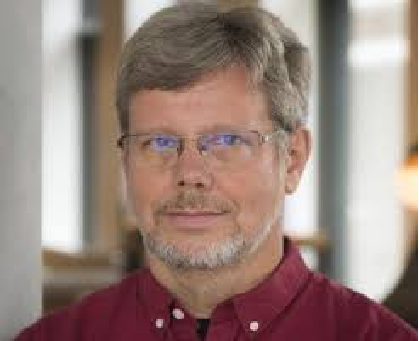
\includegraphics[width=0.7\linewidth]{screenshot005}
	\caption[Guido van Rossum]{Guido van Rossum}{image via:thefamouspeople.com}
	\label{fig:screenshot005}
\end{figure}

\newpage

\section{APPLICATIONS OF PYTHON}
        \ Python has a part to play in developing websites and software. It is mainly used in areas like data analysis, data visualization and task automation. Python can be used in different areas of application development, such as; Web Development, Game Development, Software Development, Business Applications and even Language Development.
        It is a well known fact that in making a good software application multiple programming languages need to be utilized.Some of these software applications are:

\begin{figure}[h]
	\includegraphics[width=0.7\linewidth]{"screenshot 6"}
	\caption{}
	\label{fig:screenshot-6}
\end{figure}

\newpage

\subsection{IDEs that support python}
           \begin{itemize}
           	\item PyCharm
           	\item Spyder
           	\item Vim
           	\item Atom
           	\item Pydev
           \end{itemize}
       
\begin{figure}[h]
	
\includegraphics[width=0.7\linewidth]{screenshot006}
	\caption{image via:datacamp.com}
	\label{fig:screenshot006}
\end{figure}

\newpage

\subsubsection{Programming languages related to python}
              \begin{itemize}
              	\item Ruby
              	\item PHP
              	\item Java
              	\item Golang
              	\item Scala
              \end{itemize}
          
\newpage

\section{C++}

\subsection{HISTORY}
           \begin{itemize}
           	\item Bjarne Strousup was the programmer that developed C++.
           	\item It was initially built upon the C programming language. 
           	\item He later named it C++ after various improvements.
           \end{itemize} 

\begin{figure}[h]
	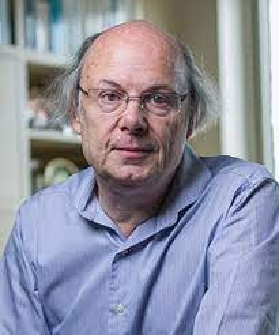
\includegraphics[width=0.7\linewidth]{screenshot007}
	\caption{Bjarne Stroustrup}{image via:stroustrup.com}
	\label{fig:screenshot007}
\end{figure}

\newpage

\subsection{APPLICATIONS OF C++}
           \ C++ programming language can be applied in the development of operating        systems,Game development and large scale web applications. C++ has been applied in software applications like:
           
\begin{figure}[h]
	
\includegraphics[width=0.7\linewidth]{screenshot008}
	\caption{}
	\label{fig:screenshot008}
\end{figure}

\newpage

\subsection{IDEs that support C++:}
           \begin{itemize}
           	\item Eclipse
           	\item Visual Studio Code
           	\item CodeLite
           	\item CLion
           \end{itemize}

\begin{figure}[h]
	\includegraphics[width=0.7\linewidth]{"9th pic"}
	\caption{}
	\label{fig:9th-pic}
\end{figure}

\newpage

\subsection{Programming languages related to C++}
           \begin{itemize}
           	\item Python
           	\item C-sharp
           	\item Java
           	\item Rust
           	\item Golang
           \end{itemize}


\newpage

\section{Java}
\subsection{HISTORY}
           \ James Gosling developed Java in 1995.It originally started as project oak by James in June 1991. James was not  the only one that had a part to play in the development of Java, he had colleagues that worked with him at Sun Microsystems.
           
           
\begin{figure}[h]
	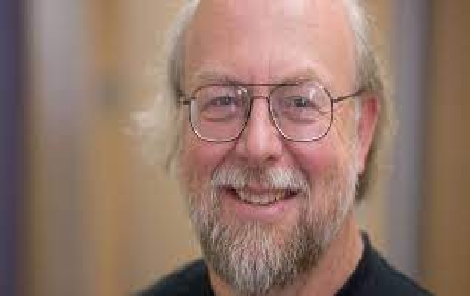
\includegraphics[width=0.7\linewidth]{screenshot009}
	\caption{James Gosling}{Image via:wealthypersons.com}
	\label{fig:screenshot009}
\end{figure}

\newpage

\subsection{APPLICATIONS OF JAVA:}
           \ Java can be applied in the development of gaming applications,web-based applications and even mobile development. Examples of software applications that have been developed with Java are:
           
\begin{figure}[h]
	
\includegraphics[width=0.7\linewidth]{screenshot010}
	\caption{}
	\label{fig:screenshot010}
\end{figure}

\newpage

\subsection{IDEs that support Java:}
           \begin{itemize}
           	\item Kite
           	\item Apache NetBeans
           	\item Xcode
           	\item BlueJ
           	\item IntelliJ IDEA
           \end{itemize}

\begin{figure}[h]
	
\includegraphics[width=0.7\linewidth]{screenshot011}
	\caption{}
	\label{fig:screenshot011}
\end{figure}

\newpage

\subsection{Related programming languages to Java}
           \begin{itemize}
           	\item C-sharp
           	\item Ruby
           	\item Small talk
           	\item Lisp
           \end{itemize}


\newpage

\section{JavaScript}
\subsection{HISTORY}
           \ Brendan Eich created JavaScript.This happened in 1995.Brendan developed the language with the help of netscape communications. It was originally created as a scripting language that could be used on Netscapes web browser.
           
\begin{figure}[h]
	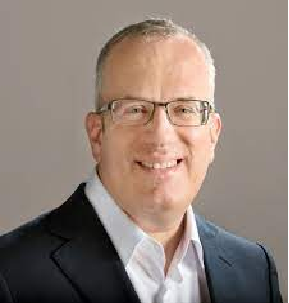
\includegraphics[width=0.7\linewidth]{screenshot012}
	\caption{Brendan Eich}{Image via:en.wikipedia.org}
	\label{fig:screenshot012}
\end{figure}

\newpage

\subsection{APPLICATIONS OF JAVASCRIPT}
           \ Javascript is used in the development of websites, it can also be used in development of web servers and game development.Examples of applications which use JavaScript are:
           
           
\begin{figure}[h]
	
\includegraphics[width=0.7\linewidth]{screenshot013}
	\caption{image via:appventurez.com}
	\label{fig:screenshot013}
\end{figure}

\newpage

\subsection{IDEs that support JavaScript}
           \begin{itemize}
           	\item WebStorm
           	\item Visual Studio Code
           	\item Atom IDE
           	\item Brackets
           \end{itemize}

\begin{figure}[h]
	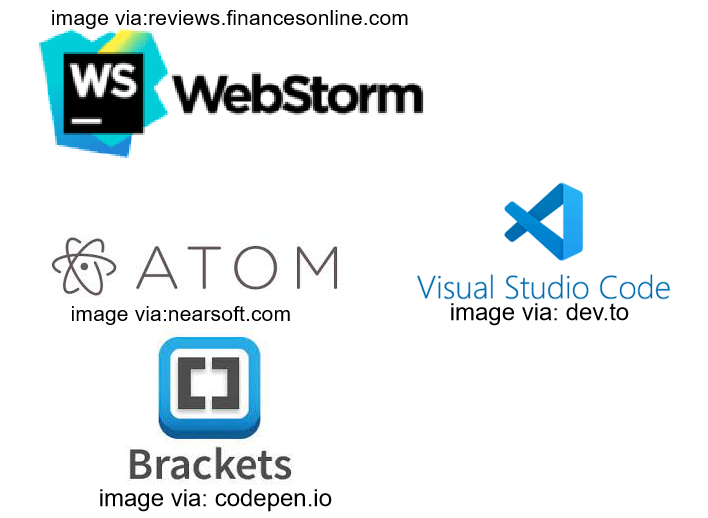
\includegraphics[width=0.7\linewidth]{screenshot014}
	\caption{}
	\label{fig:screenshot014}
\end{figure}

\newpage

\subsection{Programming languages related to JavaScript}
           \begin{itemize}
           	\item Dart
           	\item CoffeeScript
           	\item Opal
           	\item Kaffeine
           	\item Roy
           \end{itemize}

\newpage

\subsection{HTML}
\subsubsection{HISTORY}
        \ Sir Tim Berners-Lee created the Hypertext Markup Language. He created it in 1991. It was released in 1995 as HTML 2.0. HTML was created so that pages could be created on the World Wide Web using text.
        
\begin{figure}[h]
	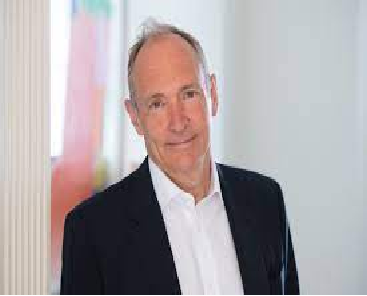
\includegraphics[width=0.7\linewidth]{screenshot015}
	\caption{SIR TIM BERNERS-LEE}{Image via:w3.org}
	\label{fig:screenshot015}
\end{figure}

\newpage

\subsection{APPLICATIONS OF HTML:}
           \  HTML is primarily known for the part it plays in web page development. It can also be used in Data entry and Internet Navigation.
           
\newpage

\subsection{IDEs that support HTML}
           \begin{itemize}
           	\item Visual Studio
           	\item IntelliJ IDEA
           	\item Komodo IDE
           	\item Sublime Text 3
           	\item Eclipse IDE
           \end{itemize}
       
\begin{figure}[h]
	
\includegraphics[width=0.7\linewidth]{screenshot016}
	\caption{}
	\label{fig:screenshot016}
\end{figure}






\end{document}
